\chapter{Background - 30\%}


\begin{itemize}
    \item Literature Review
    \item Summary of similar systems to yours
    \item Explanations of concepts that you will rely on later
    \item Advantages and Disadvatages of different approaches
    \item Point out problems that you are going to improve on
    \item Cite all of your references
\end{itemize}

Function merging is a powerful code optimisation technique that reduces redundancy by combining similar or identical functions within a program. This shrinks the code size and potentially improves performance. At its core, function merging involves identifying functions with similar structures and semantics, and then creating a merged function that preserves the behaviour of each original function.

Typically, the process begins with analysing pairs or groups of functions to identify regions of similarity. After identifying these similarities, a merged function is constructed that uses parameters to determine which behaviour should be executed. This unified function incorporates decision points—often implemented as conditional branches—that select the appropriate logic path based on the input parameters. In doing so, the merged function maintains the distinct functionality of the original functions while eliminating redundant code.

\section{LLVM}
\subsection{LLVM IR} \label{LLVM:IR}
IR is SSA - Single static assignment or whatever
\subsection{LLVM Bitcode} \label{LLVM:Bitcode}



\section{Compiler}
Compilers serve as translators that convert high-level programming languages into machine-executable code. Their goal is to produce the most efficient executable code where possible while still preserving semantic correctness. Modern compilers work by performing numerous analyses and transformations to improve the code quality.

The compilation process can be broadly split into three stages, the front-end, the middle-end and the back-end. The front-end is responsible for lexical analysis, parsing, and semantic analysis to convert source code into an intermediate representation (IR). The IR serves as a language and target independent abstraction of the program. By using an IR, developers can reduce the work needed to add support for a new source language or target, only the connection to the IR must be implemented rather than a completely new pipeline for every other existing target or source. Next, the middle-end analyses and optimises the IR where possible. Finally, the back-end transforms the optimised IR into target-specific machine code through instruction selection, register allocation, and more.

In modern compilers, optimisations are organised into passes, each concentrating on one type of optimisation. The function merging pass described in this paper is located in the middle-end, operating on the IR during link time optimisation (LTO). LTO allows the compiler to view and optimise the entire program as a unified whole rather than as isolated modules, allowing optimisations across module boundaries. This whole-program visibility enables optimisations to work across module boundaries that would normally be isolated. For function merging especially, LTO provides access to all functions across the program, substantially increasing opportunities for identifying and combining similar code \cite{FunctionMergingSequenceAlignment}. 

This project is built upon a state-of-the-art (SOTA) implementation of function merging, F3M \cite{F3M:FastFocusedFunctionMerging},  which was implemented in LLVM, a compiler toolchain. The modular pass-based architecture of LLVM makes it ideal for integrating the project into the pipeline without too much complexity. Additionally, LLVM is widely used across industry and academia, meaning that it has support for many high-level languages and target architectures, ensuring that optimisation can have a broad practical impact.

\section{Related Work}
In this chapter, we will talk about previous solutions to function merging and the current function merging technique used in LLVM at the moment. Function merging is still an actively researched pass in compilers, trying to analyse the best methods to analyse pairs of functions which will merge well and how to do the merging as well.

\subsection{LLVM Function Merging}
Currently in LLVM, a conservative implementation of two-phase function merging exists, emphasising efficiency over comprehensive merging opportunities. The implementation first categorises functions using a lightweight hash-based approach before performing a detailed comparison between functions with matching hash values \cite{LLVMFuncMergSrc}.

\subsubsection{Hashing}
The hashing phase efficiently groups potential merge candidates by capturing structural similarities while maintaining the invariant:

\begin{equation}
F1 == F2 \Rightarrow Hash(F1) == Hash(F2)
\end{equation}

It is therefore guaranteed that if two functions are the same, they will hash to the same value. This hash function accounts for function signatures, control flow structure, and instruction opcodes. Only functions producing identical hash values proceed to the detailed comparison phase, which examines their basic blocks and instructions to confirm mergability based on matching operations and compatible operand types.

\subsubsection{Limitations}
The existing approach is inherently conservative, primarily targeting functions with nearly identical control flow graphs and instruction sequences \cite{LLVMMergeFunctionsPass}. While it does accommodate cases where operand types differ but can be safely bitcasted between each other, this flexibility is quite limited. This conservative stance significantly limits merging opportunities, particularly for functions that contain substantial shared code but differ in specific regions. The current implementation misses potentially valuable merging candidates where functions have similar but not identical structures, cases where merging could yield significant code size benefits by consolidating redundant sections while branching at divergent points.

These limitations establish a clear opportunity for more sophisticated merging decision mechanisms that can recognise non-obvious structural similarities and better predict optimisation benefits.

\subsection{Function Merging by Sequence Alignment (FMSA)}
Rocha et al. introduced a novel technique for code size reduction that adapts sequence alignment algorithms from bioinformatics to merge similar functions \cite{FunctionMergingSequenceAlignment}. This technique attempts to address a limitation of previous methods, either merging almost identical functions or algorithms which struggled to identify feasible functions for merging.

This approach consists of three stages, function linearisation, sequence alignment and code generation. During linearisation, the functions are transformed by traversing the function's blocks in the control-flow graph (CFG). The basic blocks and labels are then expanded where necessary to produce the linearised function consisting of instructions. 

Next, the algorithm leverages the Needleman-Wunsch algorithm to align instruction sequences, which was originally developed for identifying similarities between amino acids of proteins. This dynamic programming algorithm assesses two linearised functions to identify regions of similarity by inserting blank objects where necessary to maximise matching between equivalent segments. 

\begin{figure}[tbh!]
\centering
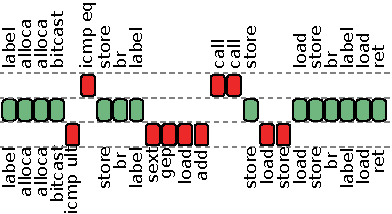
\includegraphics[scale=1]{Figures/FMSA_FunctionSA.pdf}
\caption{The sequence alignment between two functions, identifying the equivalent segments of code (green in the center) and the non-equivalent ones (red at the sides). Figure and caption taken from \cite{FunctionMergingSequenceAlignment}.}\label{fig:SequenceAlignment2Funcs}
\end{figure}

For this to work, criteria were chosen to determine when two instructions are considered to be matching. They are considered matching when they have semantically identical opcodes, equivalent result types and pairwise equivalent operand types. Types are considered equivalent when they can be bitcasted between each other losslessly.

In the final code generation stage, the aligned instruction segments with equivalent code are merged, while non-equivalent segments are maintained but guarded by a function identifier parameter that is added to the merged function.

% \begin{figure}[tbh!]
% \centering
% 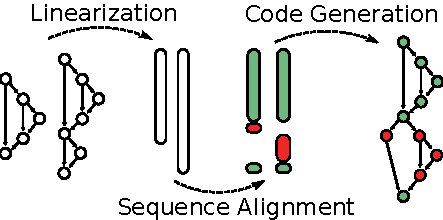
\includegraphics[scale=1]{Figures/FMSA_Technique.pdf}
% \caption{ Overview of function-merging by sequence alignment. Equivalent segments of code is represented in light green and the non-equivalent ones in dark red \cite{FunctionMergingSequenceAlignment}.}\label{fig:testsvg}
% \end{figure}

This technique demonstrated amazing results, reducing code size by 25\% on Intel architecture and 30\% on ARM. Approximately 2 times better than the state-of-the-art at the time.

\subsubsection{Alignment Score} \label{METRIC:AlignmentScore}
The sequence alignment between two functions is a property that identifies the structural similarity between two functions, serving as a key predictor of function merging profitability. This provides direct insight into how effectively two functions can be merged and is the characteristic our machine learning model aims to predict.
To quantify this value, the alignment score metric is used, defined as the ratio of the number of aligned instructions to the total number of instructions:
$$Alignment\ Score = \frac{Number\ of\ Aligned\ Instructions}{Total\ Aligned\ and\ Unaligned\ Instructions}$$
Using figure \ref{fig:SequenceAlignment2Funcs} we can calculate the alignment score as follows:
$$\frac{No.\ of\ Green\ Nodes}{Total\ No.\ of\ Green\ and\ Red\ Nodes}=\frac{14}{24} = 0.5833$$

Given that this metric is a ratio, this metric will be a continuous value in the range of [0, 1] inclusive, where 0 represents a completely dissimilar function pair and 1 representing a structurally identical function pair.


% \subsection{HyFM}
% HyFM is a notable function merging algorithm developed to solve the issue of the time needed to compiler code. Previous advanced function merging implementations were quadratic in complexity with regards to the number of functions. On top of that, the implementations were too keen on merging all selected functions, where most of the time the merged functions were unprofitable.\cite{HyFM:FunctionMergingForFree}

% \subsubsection{Basic Blocks}
% HyFM works at the basic block level, where basic blocks are blocks of instructions which are executed sequential, there are no branches. Since basic blocks are must shorter than functions, the alignment time is negligible compared to the time needed for attempting to align functions. By analysing how well basic blocks align with each other, the algorithm has an early sense of how well two functions align before attempting the alignment, saving time and resources from attempting unprofitable pairs.

% A fingerprint is generated for every basic block, and the basic blocks with the shortest distance between their fingerprints are considered good.
% If a pair of basic blocks are estimated to benefit from merging, it is then passes onto the more expensive merging phase.

% \subsection{Benefits}
% HyFM is able to decrease the alignment score

% \subsection{F3M: Fast Focuses Function Merging}

% \section{Quantifying Semantics}

% \subsection{Word2Vec}
% \subsection{IR2Vec}

\subsection{HyFM}
HyFM tries to tackle the inefficiencies of the previous state-of-the-art (SOTA) by introducing multiple optimisations \cite{HyFM:FunctionMergingForFree}. 

\subsubsection{Basic-Block Granularity} \label{HyFM:BasicBlockGranularity}
First, HyFM works at the basic-block level instead of function level. While the complexity is still $O(n^2)$ for the Needleman-Wunsch (NW)algorithm, $n$ in the previous SOTA refers to the number of instructions in functions whereas $n$ in HyFM refers to the number of instructions in basic blocks, which is considerably smaller, resulting in a dramatic memory reduction.

\subsection{Fingerprint} \label{HyFM:FingerprintDistance}
Before performing alignment, HyFM uses fingerprints to efficiently identify similar blocks. Each fingerprint is a fixed-size vector representing the frequency count of each opcode in a block. HyFM pre-computes fingerprints for all basic blocks and uses the Manhattan distance between these fingerprints to pair similar blocks from different functions. This lightweight filtering mechanism helps HyFM quickly focus on promising block pairs before applying the more expensive alignment analysis.


\subsubsection{Pairwise-Alignment (PA)} \label{HyFM:PairwiseAlignment}
Additionally, HyFM introduces a new linear-complexity pairwise alignment (PA) strategy that only aligns instructions in corresponding positions, with instructions matching only if they have the same opcode. It has been identified that most basic blocks that would be profitably merged have highly similar structure, making this simpler approach effective for real-world code. Finally, HyFM implements a multi-tiered profitability analysis, allowing it to bail out early from unprofitable and expensive merging attempts. This prevents wasting resources on generating merged code that would ultimately be discarded, contributing to HyFM's speedup compared to the previous SOTA.

\subsection{F3M: Fast Focused Function Merging}
This project is built on the current state-of-the-art function merging, Fast Focused Function Merging's (F3M) infrastructure. F3M represents the current state-of-the-art in function merging technology to address critical inefficiencies that previously made function merging impractical for large-scale applications. While its predecessor, HyFM, improved function merging by operating at the basic block level \cite{HyFM:FunctionMergingForFree}, F3M introduces fundamental innovations that dramatically reduce compilation time while maintaining or improving code size reduction.

The technique introduces two key innovations. First, F3M employs MinHash-based fingerprinting that better captures the semantic similarity between functions. 

\subsubsection{Min-Hash Fingerprinting} \label{METRIC: MinHashFingerprint}
Each instruction is encoded as a 32-bit integer representing four critical properties: opcode, result type, number of operands, and operand types. These encoded instructions are then grouped into overlapping "shingles" (pairs of consecutive instructions).  Multiple hash functions are then applied to each shingle, with only the minimum hash value across all shingles from each function retained, producing a fixed-length fingerprint vector.

\begin{figure}[h!]
\centering
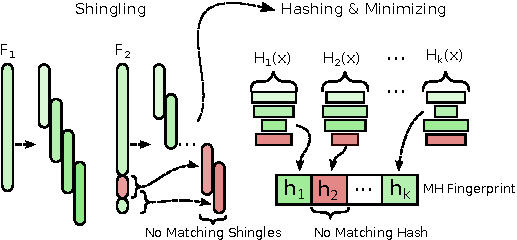
\includegraphics[scale=1]{Figures/F3M_MinHash.pdf}
\caption{The MinHash algorithm: Textual documents are broken up into overlapping subsequences; Each subsequence is hashed with k different hash functions; For each function, the smallest hash is saved creating a fingerprint of k entries. In this example, two functions differ in only a couple extra instructions inside F2. For F2’s fingerprint, this creates shingles and hashes with no matches in F1, representing the slight difference between them. Figure and caption taken from  \cite{F3M:FastFocusedFunctionMerging}.}\label{fig:testsvg}
\end{figure}

\subsubsection{Comparing MinHash Fingerprints} \label{METRIC:MinHashDistance}
To compare the MinHash fingerprints, the Jaccard Index between two fingerprints is calculated, representing the likelihood of matching instruction subsequences. For two fingerprints A and B, the index is calculated by finding the ratio of identical pairwise hash values compared to the total number of hashes ($k$):

$$J(A, B) = \frac{|A\cap B|}{k}$$

The Jaccard distance is then computed as: 
$$d(A, B) = 1 - J(A, B)$$

\subsubsection{Locality Sensitive Hashing (LSH)}
Second, F3M implements Locality Sensitive Hashing (LSH) to drastically reduce the search complexity from quadratic to near-linear. Rather than comparing every function against every other function, LSH divides each fingerprint into multiple bands (groups of hash values) and then maps each band to buckets in a hashmap. Only functions that share at least one bucket are considered for detailed similarity analysis, cutting down the amount of similarity analysis needed to be done.

% \begin{figure}[tbh!]
% \centering
% 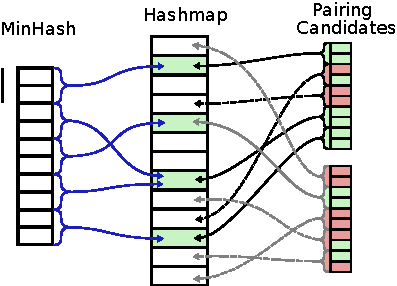
\includegraphics[scale=1]{Figures/F3M_LSH.pdf}
% \caption{ LSH - Similar sequences hashing to the same buckets. Three fingerprints
% with 10 hashes each, setting b to 5 and r to 2. References to each item are
% placed in each of their respective buckets. Since they share at least one of
% their bands they will be compared during candidate lookup \cite{F3M:FastFocusedFunctionMerging}.}\label{fig:testsvg}
% \end{figure}

\todo {INCLUDE SECTION/IMAGE ON HOW THE FUNCTIONS GET MERGED}


F3M was able to reduce the code size by a further $6\%$ on average while being able to reduce the compile time by $1.8\times$ on average across a wide range of benchmarks. Additionally, this shows the importance of the when-to-merge heuristics on the performance. Although F3M performs very well, especially for the amount of time needed to compile, the model is still very dependent on handcrafted heuristics that use fixed encoding schemes and statically determined parameters. These preset rules cannot adapt to different code patterns or contexts, and may not recognise all the patterns which indicate a suitable match.



\section{Machine Learning} \label{ML}
Machine learning (ML) offers an alternative by shifting from explicitly programmed rules to data-driven decision models. A machine learning model is a mathematical model with parameters that is tuned using data. The fundamental advantage of ML-based approaches lies in their ability to discover and leverage intricate patterns across multiple dimensions of code structure and behaviour.

\subsection{Supervised Learning}
There are multiple machine learning paradigms, each classified by the way they learn from their data and whether the expected output is provided.

Supervised learning is a machine learning paradigm in which learning is guided by labelled data \cite{MLParadigms} \cite{SupervisedLearningAndTrainingProcess}. In this approach, each input example is paired with a corresponding output, allowing the model to learn a mapping from inputs to outputs through the minimisation of a defined loss function. This process often involves iterative optimisation techniques to adjust model parameters and improve prediction accuracy. 

This supervised approach is more appropriate than alternatives like unsupervised learning, which typically operates by identifying similar data points through clustering or pattern recognition techniques. While unsupervised learning can identify similar functions, it is not quantify merging benefits.

For function merging optimisation, supervised learning enables a model to predict the profitability of merging two functions by training on examples of previously merged functions and their alignment score. In our context, the labelled data consists of pairs of functions and their corresponding alignment score.

\subsection{Loss Function} \label{ML:LossFunction}
A loss function, also known as cost or error function, is a mathematical function that quantifies the difference between the model's current predicted value and the ground truth (actual values).

Loss functions fall into two primary categories corresponding to the tasks, regression models (predicting values on a continuous spectrum) and classification models (selecting a value from a discrete set of values). For this paper we will be focusing on regression loss functions to predict the alignment score for a pair of functions, further discussed in section  \ref{METRIC:AlignmentScore}, allowing the estimate of merging benefits without expensive computations.

\subsubsection{Mean Squared Error (MSE)}
Mean squared error is a widely used loss function for regression tasks. It is derived by the following formula: 
$$MSE=\frac{\sum^n_{i=1}(y_i-\hat{y}_i)^2}{n}$$

\hspace{1cm} $y_i = $ Ground Truth Value

\hspace{1cm} $\hat{y}_i = $ Predicted Value

\hspace{1cm} $n = $ Number of Samples

The squaring operation in MSE provides two benefits. First, it makes all errors positive, ensuring that when multiple errors are combined and averaged in a batch, positive and negative errors do not cancel each other out, providing a true measure of error. Second, it emphasises larger errors due to the quadratic nature of the function. This emphasis prioritises the reduction of substantial prediction errors before fine-tuning smaller discrepancies—a desirable property when approximate predictions in the correct range, especially important when dealing with small values in the range of 0-1.

A smaller MSE is better, signifying reduced discrepancy between the predicted value and the ground truth. For our function merging application, MSE is preferable to alternatives like Mean Absolute Error (MAE) because the quadratic penalty helps the model focus on avoiding large prediction errors that could lead to poor merging decisions.

% \subsubsection{Mean Absolute Error (MAE)}

\subsection{Gradient Descent} \label{ML:Gradients}
The derivative of a function $f$, given by $\frac{df}{dx}$ measures the sensitivity of a function to change in the output given a certain input. This rate of change is also known as a function's gradient; geometrically, the slope of the tangent to the function's plot at a certain input. 

Gradient descent, the primary optimisation algorithm in deep learning, involves two stages, forward propagation and backward propagation. During \textbf{forward  propagation}, the model processes the training data through itself to produce a set of predictions. The loss function then quantifies the error between these predictions and the ground truth.

During \textbf{backward propagation}, the gradient for the loss function is calculated with respect to each parameter in the model using the chain rule. The gradients indicate the direction and magnitude of parameter adjustment needed to reduce the loss. Each parameter then is adjusted in the opposite direction of the gradient, scaled by the selected learning rate, discussed in section \ref{ML:LearningRate}.  This process iteratively navigates the parameter space toward a local minima of the loss function if it is well designed. In practice, finding a global minima is not always possible, so a well suited local minima is sufficient for predictions.

The objective of all gradient descent methods is to minimise the loss function, iteratively refining the model to make predictions that more closely match the ground truth.

% \subsection{Training}
% Learning is a process to acquire expertise or knowledge about a domain through experience and practice \cite{LearningDefinition1}\cite{LearningDefinition2}. The training process follows the following cycle \cite{DeepLearningGoodfellow}:
% \begin{enumerate}
%     \item \textbf{Forward Propagation}: The model processes a batch of input samples through it's layers using the current parameters.
%     \item \textbf{Loss Calculation}: The loss function quantifies the error between the model's predictions and ground truth.
%     \item \textbf{Backward Propagation}: The gradients of the model's loss is calculated with respect to its parameters using the chain rule.
%     \item \textbf{Parameter Update}: An optimisation algorithm adjusts the parameters in the opposite direction of the gradient to reduce the loss.
% \end{enumerate}
% This process is repeated until a stopping criteria is met.

\subsection{Hyperparameters}
A ML model usually has hyperparameters to configure. These are model parameters which are not learnt, and are configured before a model starts training. Unlike model weights which are optimised during training, hyperparameters control the learning process itself. They control how the model learns and behaves from the input data. A subset of the dataset, called the validation set, is usually set aside to tune the hyperparameters. Some of the most common hyperparameters are discussed below.

\paragraph{Epochs} \label{ML:Epochs} The epoch specifies the number of times the model trains using the entire training data. Setting a value that is too low may cause the model to underfit\footnote{\textbf{Underfitting} - When a model is unable to capture the underlying patterns in the training data, leading to poor performance on training and unseen data} to the training data, while a value that is too high may cause the model to overfit\footnote{\textbf{Overfitting} - When a model starts memorising the training data, capturing noise and irrelevant information instead of trying to learn the patterns associated with the data leading to poor generalisation on unseen data} to the training data, causing a drop in performance when evaluated against the validation set. One way to prevent overfitting due to excessive epochs is by implementing early stopping. Early stopping addresses this by monitoring the model's performance on the validation data, and halting training when the validation performance degrades, preventing overfitting.

\paragraph{Learning Rate} \label{ML:LearningRate} The learning rate determines the size of the step taken by the model for each training iteration. Selecting a large value means less time is needed for training, but the model may overshoot the global minimum and struggle to converge. On the other hand, if the learning rate is too small, the model will converge on a local minimum and not be able to leave it, thus not finding the optimal solution. Adaptive learning rate techniques like Adam can adjust the learning rate dynamically during training to improve the convergence.

\paragraph{Batch Size} \label{ML:BatchSize} The batch size specifies the number of training samples processed in each training iteration. The loss and gradient is averaged for all training samples in a batch. Selecting a suitable batch size is important, one too small will cause the model to not converge on the right direction as it will account for all the noise, one too big and it will require more memory for training and converge to a suboptimal solution.


\paragraph{Hyperparameter Optimisation} Since hyperparameters can greatly affect a model's training, it is important to find a suitable value for the model and task. There are multiple ways to do this, including manually running experiments or Bayesian optimisation. Bayesian optimisation works by constructing a probabilistic model of the objective function and using it to select the most promising hyperparameters to evaluate next. 

\subsection{Imbalanced Dataset}
In a perfect world, a dataset will have a similar amount of data samples for across the output data's range/spectrum, but this is not always possible. If no effort is taken to take into account the imbalance of the data samples, a model will learn to predict more of the dominant data samples. To mitigate this, sample weightings can be used, where it will scale down the loss for the dominant data points and scale up the loss for under-represented data points, this is known as \textbf{cost-sensitive learning (weighting)} \cite{ImbalancedDataset}. This ensures that the loss function will adjust the parameter in a reasonable manner without overfitting itself to predict more for the dominant data points.

% \subsection{Testing}
% Finally, another third subset of the dataset is set aside to evaluate the model's overall performance, known as the testing set. It is crucial that this set of data has not been used or seen at all by the model, so that the model's final evaluation can be unbiased on its ability to generalise to unseen data. The subsets of data that have been discussed so far, training, validation and testing should all be divided up at the start before model training to prevent data from training to be used for evaluation or vice versa. For regression tasks, mean-squared error (MSE), mean absolute error (MAE) and mean absolute percentage error (MAPE) are popular options. The MSE was selected as the metric because it emphasises larger errors, especially important when we are dealing with such small numbers and the MAPE is unable to deal with ground truth values that are 0 as division with 0 is not possible.

\subsection{Other Applications of ML in compilers}

% \subsubsection{Optimisation Selection}
% Optimisation selection determines which compiler optimisations should be applied to a program to achieve the best performance, code size, or other objectives. Compilers typically have dozens or hundreds of individual optimisation passes available, each with various parameters and settings. \todo{CITE Optimisation SELECTION}

% The challenge lies in deciding which optimisations to apply to a particular program, in what order, and with what parameters. Traditionally, compilers use predefined heuristics based on fixed rules established by compiler developers. However, these heuristics often fail to capture the complex interactions between optimisations and program characteristics across different architectures.

% Optimisation selection using machine learning has emerged as a powerful approach to automate compiler optimisations. MILEPOST GCC represents one of the pioneering efforts in this area, automatically adjusting compiler optimisation heuristics to improve execution time, code size, or compilation time \cite{OptimisationSelectionML}. The system collects program features and execution feedback and then uses this data to train models that predict optimisation strategies for new programs. This approach eliminates the need for expert hand-tuning of optimisation heuristics for each new architecture or program. Experimental results showed that MILEPOST GCC could reduce the execution time of the MiBench benchmark suite on the ARC processor architecture.

% The key innovation of this approach is that it replaces static, hardwired compiler optimisation decisions with data-driven models that can adapt to different architecture characteristics. This makes porting optimisation compilers to new hardware significantly more efficient, as the system automatically learns appropriate optimisation strategies rather than requiring manual recalibration.

% \subsubsection{Iterative Compilations}
% Iterative compilation is a technique that repeatedly compiles a program with different optimisation settings and evaluates the resulting performance to find the best configuration. Rather than relying on heuristics to determine the optimal optimisation strategy upfront, iterative compilation empirically explores the space of possible optimisations. \todo{CITE ITERATIVE COMPILATION}
% Iterative compilation traditionally requires extensive and repetitive fine-tuning to find optimal compiler optimisations, which creates a significant bottleneck in the development process. This challenge is addressed by applying active learning techniques to minimise the cost of iterative compilation \cite{IterativeCompilationWActiveLearningML}.
% The research demonstrated that traditional iterative compilation wastes substantial effort collecting redundant training data. Many of the performance measurements collected contribute little to the final optimisation heuristic. Their approach optimised both the selection of training examples and the number of samples per example using sequential analysis.

% By applying active learning principles, their methodology reduced training overhead compared to approaches with fixed sampling plans. The system determines dynamically whether additional samples are needed for a particular configuration based on the current model's uncertainty. This transforms what would typically take months of compilation and performance measurements into days, making machine learning-based compilation much more practical for real-world deployment.

% \subsubsection{Loop Vectorisation}
% Loop vectorisation is a compiler optimisation technique that transforms sequential loop operations to take advantage of modern processors' SIMD (Single Instruction, Multiple Data) capabilities. Instead of processing one data element per instruction, vectorisation allows a single instruction to simultaneously operate on multiple data elements. \todo{CITE LOOP VECTORISATION}

% Loop vectorisation is a critical compiler optimisation for modern SIMD-compatible architectures. NeuroVectorizer represents a significant advance in this area by using deep reinforcement learning to predict optimal vectorisation factors for loops \cite{LoopVectorisationML}.

% Traditional vectorisers in compilers like LLVM use fixed-cost models based on heuristics to make vectorisation decisions. These models struggle to accurately capture data dependencies, computation graphs, and instruction organisations. NeuroVectorizer takes a fundamentally different approach by employing a neural network that learns code embeddings directly from loop source code and then uses reinforcement learning to determine the optimal vectorisation and interleaving factors.

% The system achieved impressive results, showing performance speedup compared to the baseline LLVM vectoriser across various benchmarks. The reinforcement learning model proved particularly effective because it can learn complex patterns from code structure without requiring explicit feature engineering and can co-optimise multiple objectives like execution time and code size simultaneously.

% \subsubsection{Function Inlining}
% Function inlining is a compiler optimisation that replaces a function call with the called function's actual body. This eliminates the overhead of the function call mechanism (saving the registers, jumping to the function code, returning, and more) \todo{CITE Function Inlining}. MLGOPerf extends machine learning approaches to function inlining decisions in LLVM \cite{FunctionInliningML}.

% While MLGO (Machine Learning Guided Optimisation) previously focused on optimising code size with ML-based inlining, MLGOPerf specifically targets performance optimisation. The system employs two ML models: a primary reinforcement learning model that makes inlining decisions and a secondary model (IR2Perf) that predicts post-inlining speedup to generate rewards for training the RL agent.
% This two-model approach enables fast training without requiring the time-consuming execution of actual programs for each training iteration. Experimental results showed that MLGOPerf improved performance over LLVM's O3 optimisation level on SPEC CPU2006 and Cbench benchmarks. 
% Function inlining optimisation represents a particularly challenging problem due to the exponential growth of the optimisation space, making machine learning approaches especially valuable in this domain.

\paragraph{Optimisation Selection} Optimisation Selection focuses on determining which compiler optimisations to apply to a program to enhance performance, reduce code size, or meet other objectives. Traditionally, compilers have relied on fixed rule-based heuristics developed by compiler engineers to choose from a vast array of optimisation passes. However, with techniques like those used in MILEPOST GCC, machine learning models now collect program features and runtime feedback to automatically predict the most beneficial optimisation strategies, thereby replacing static rules with adaptable, data-driven decisions. This not only streamlines the optimisation process for various architectures but also reduces the need for manual tuning by experts \cite{OptimisationSelectionML}.

\paragraph{Iterative Compilation} Iterative Compilation tackles the optimisation challenge by repeatedly compiling a program with different settings and empirically testing the resulting performance. Instead of depending solely on predefined heuristics, this method explores a broader range of optimisation configurations to identify the optimal solution. The process is enhanced by active learning strategies which intelligently select training examples and adjust sampling dynamically based on the model's uncertainty. This adaptive approach dramatically reduces the time and effort required for extensive fine-tuning \cite{IterativeCompilationWActiveLearningML}.

\paragraph{Loop Vectorisation} Loop Vectorisation is a compiler optimisation that transforms sequential loop operations to exploit the parallel processing capabilities of SIMD hardware. Traditional vectorisers use fixed-cost heuristic models that may not fully capture the complex data dependencies and instruction patterns within code loops. In contrast, advanced approaches like NeuroVectorizer use deep reinforcement learning to predict the best vectorisation factors for loops. This method learns code representations directly from the source code, allowing it to determine more effective vectorisation and interleaving factors, which in turn leads to significant performance improvements over conventional heuristic models \cite{LoopVectorisationML}.

\paragraph{Function Inlining} Function Inlining is a technique that replaces a function call with the body of the function itself, thereby eliminating the overhead associated with calling a function. Recent advances, such as MLGOPerf, extend machine learning techniques to optimise inlining decisions. This approach leverages a two-model strategy: a primary reinforcement learning model for decision making and a secondary model to predict the performance gains from inlining. By doing so, the system efficiently optimises inlining, and has demonstrated improvements in performance on standard benchmarks compared to traditional inlining strategies \cite{FunctionInliningML}.

% \begin{itemize}
%     \item Optimisation Selection \cite{OptimisationSelectionML}
%     \item Iterative Compilation using Active Learning \cite{IterativeCompilationWActiveLearningML}
%     \item Loop Vectorisation \cite{LoopVectorisationML}
%     \item Function Inlining \cite{FunctionInliningML}
    
% \end{itemize}

\section{Neural Networks}
Neural networks represent a specialised and powerful class of machine learning models inspired by the structure and function of the human brain. While traditional machine learning approaches often rely on carefully engineered features and may struggle with complex, high-dimensional data, neural networks excel at automatically learning hierarchical representations from raw inputs.

The foundation of a neural network consists of \textbf{artificial neurons}, a mathematical function that mimics the basic behaviour of a biological neuron. Each artificial neuron receives one or more input signals, multiplies them by their corresponding weight, sum up the values, adds a bias term, and then passes the result through a non-linear activation function to produce an output signal.

% TODO: Add picture of artificial neuron

The overall architecture of a neural network is defined by how these neurons are arranged in layers: the \textit{input layer} accepts raw data, one or more \textit{hidden layers} perform successive transformations to extract increasingly abstract features, and the \textit{output layer} generates the final prediction. The complexity and performance of a neural network is largely influenced by its \textit{depth} (the number of layers) and its \textit{width} (the number of neurons per layer). Training is typically performed via optimisation algorithms like gradient descent and back-propagation, which adjust the network’s weights to minimise a loss function.

This automatic feature discovery and end-to-end learning process, which minimises the need for manual feature engineering, sets neural networks apart from traditional ML.

\subsection{Semantical Representations} \label{subsection:SemanticalRepresentations}
Machine learning models face a fundamental limitation when processing data, they operate exclusively on numerical values. This creates a significant challenge when working with symbolic or textual data, such as program code, natural language, or other structured representations. Since these algorithms rely on mathematical operations, inputs must be represented as numeric values or vectors; raw non-numeric data cannot be directly processed or learned from.

To overcome this limitation, the symbolic representations need to be transformed into a numerical representation which preserves it's semantic relationships and enable effective machine learning. Word embeddings serve as a prime example of this transformation, as they map words into dense, continuous vector spaces that capture semantic information.

Simple encoding techniques like \textbf{one-hot encoding}, where each unique symbol is assigned its own dimension in a vector space, fail to capture meaningful relationships between elements because all symbols are equidistant, so the encoding does not reflect any inherent similarity or dissimilarity between words. Moreover, as vocabulary size increases, one-hot encoding leads to extremely high-dimensional and sparse representations. This not only results in inefficient use of memory but also significantly increases the computational cost of training machine learning models \cite{DeepLearningGoodfellow}.

For instance, \textbf{word2vec} employs a shallow neural network with two primary architectures, the \textit{Continuous Bag-of-Words (CBOW)} model and the \textit{Skip-Gram} model \cite{Word2Vec}. In the CBOW approach, the network predicts a target word based on its surrounding context words, while the Skip-Gram model does the reverse by predicting context words given a target word. Both models learn embeddings by optimising the prediction task over a large corpus, ensuring that semantically similar words are located near each other in the resulting vector space. Similarly,  \textbf{GloVe}  was proposed as a method that leverages global word co-occurrence statistics to generate embeddings reflecting nuanced linguistic relationships \cite{GloVe}.

These embedding techniques enable machine learning models to effectively utilise the underlying semantics of the symbolic data to be able to predict on future tasks.

\subsubsection{IR2Vec} \label{subsubsec:IR2Vec}
IR2Vec is a framework that generates scalable, continuous embeddings for LLVM's Intermediate Representation (LLVM IR) \cite{IR2Vec}. Unlike traditional word embeddings that map natural language tokens into dense vector spaces, IR2Vec transforms programs and functions into vector representations by modelling the relationships among IR entities, such as opcodes, types, and operands using a translational embedding model, like \textit{TransE} \cite{TranslationalEncoding}.

This process begins by extracting relational information from the LLVM IR, which IR2Vec stores as a triplet ($<h, r, t>$). $h$ (head) represents an entity in the IR, $t$ (tail) represents another entity in the IR that has a relationship with $h$ and $r$ (relation) represents the relationship between $h$ and $t$. The triplets are then processed using a translation-based embedding model inspired by \textit{TransE}. The core idea of \textit{TransE} is that relationships should be represented by vectors such that sum of the relation vector $r$ with the head vector $h$ should approximate to the tail's vector $t$.
$$h+r\approx t$$

Relying on this concept, IR2Vec is able to build up the vector representations of the fundamental components of the IR (opcodes, operands, ...) known as \textbf{seed encoding}. These seed embeddings can then be used to build up a higher-level embeddings for higher-level program abstraction like instructions, basic blocks, functions and modules, referred to as \textit{Symbolic Encoding}.

IR2Vec offers an even richer embedding by incorporating the program's flow details, like the use-def chains and the reaching definitions, into the symbolic encoding, aptly named \textit{flow-aware encoding}. This allows the encoder to capture the program's operational semantics in addition to the syntactical information, facilitating more effective analyses and optimisations. 

\subsection{Activation Functions}
Activation functions are crucial in dense layers as they allow the network to learn non-linear relationships in the data. Common activation functions include ReLU (Rectified Linear Unit), sigmoid, and tanh, each offering different properties for gradient propagation and feature representation.
\todo{Double check this information}
\subsubsection{Sigmoid Activation Function}
\subsubsection{ReLU Activation Function}

\subsection{Layers}
In this section, the layers and techniques used by the paper will be discussed.
\subsubsection{Dense Layers}
Dense layers, also known as fully connected layers, are a fundamental building block of neural networks. In a dense layer, every artificial neuron is connected to every neuron in the preceding layer, creating a network of weighted connections. The number of neurons in a dense layer could also be treated as a hyperparameter to be tuned. A dense layer performs the following mathematical transformation:
$$y = \sigma(Wx+b)$$

\hspace{1cm}$x = $ Input vector from the previous layer

\hspace{1cm}$W = $ Weights matrix

\hspace{1cm}$b = $ Bias vector

\hspace{1cm}$\sigma =$ An activation function to introduce non-linearity

Dense layers are known for their powerful feature extraction abilities by learning complex patterns and relationships within data. They transform an input's representation into a more abstract representation. The primary advantages of dense layers include their flexibility in handling fixed-size vector inputs and their strong representational capacity. However, they can be parameter-intensive as the number of weights grows quadratically with layer width. For an input dimension of $n$ and output dimension of $m$, a dense layer requires $n \times m$ weights plus $m$ bias parameters.

This parameter intensity can lead to computational complexity and overfitting in deep networks, which is why dense layers are often used in combined with regularisation techniques, 

\subsubsection{Dropout Layer}
Regularization techniques seek to prevent overfitting by introducing controlled noise during training so that models learn representations that generalize beyond the training set. One of the most popular methods for neural networks is dropout, which directly alters the network's architecture during training instead of the usual modification of the loss function. 

At its core, dropout is very simple, each neuron in a layer is randomly deactivated on each training sample with probability $p$ (dropout rate). Equivalently, each neuron is kept with probability $q=1-p$ . During the forward pass, a binary mask $m$ of independent Bernoulli random variables is sampled and applied to the neurons, any surviving neurons are scaled by $\frac{1}{1-p}$ so that their expected value remains unchanged \cite{DropoutPaper}.

Normal neural layer's mathematical representation:
$$y = f(Wx + b)$$
After applying dropout:
$$y=f(Wx+b)\times \textbf{m}$$
There are two variants of dropout, the standard dropout which applies the scaling during inference, and inverted dropout which applies the scaling during training. Most modern frameworks use inverted dropout by default to simplify inference \cite{TensorflowDropout, PyTorchDropout}.

Typical choices for the dropout rate $p$ ranges from 0.2 to 0.5, although these values should be treated as hyperparameters and tuned for each task \cite{DropoutPaper}.

\subsubsection{Multi-Headed Attention Layers} \label{ML:AttentionMechanism}
Attention layers allow a neural network to focus on the most important feature for the current task. Not all parts of the input contribute equally to solving a problem, by learning which elements require more attention, the network can make more informed decisions. 

The attention mechanism takes in two inputs, the first input will attend to the second. There are two variants of attentions, \textbf{self-attention} where both inputs are the same so the sequence is attending to itself, or \textbf{cross-attention} where both inputs are different.

The attention mechanism starts with three learned weights used to create three vectors from the inputs, the query (Q) vector is created from the first input, and the key (K) and value (V) vectors are created from the second input. 

Then, it compares each query against all available keys to find how well each key matches the query by calculating the dot product of the pair. High-scoring pairs are given more attention while low-scoring pairs are given less attention or ignored. The scores are then put through a softmax function that converts each score into a probability. Then, the value vector is multiplied by the weight, and the elements are summed up to generate a weighted sum to produce the first input's new vector representation after attending to the second input \cite{AttentionIsAllYouNeed}.

The model then uses the newly attended vector for further processing and prediction. The error is calculated, and backpropagation is then used to update the weights to generate the Q, K and V vectors.

A multi-headed attention layer takes it one step further by having multiple attention layers in parallel to model different relationship aspects. This works by dividing the Q, K and V vector representations across the number of parallel attention mechanisms, each mechanism is known as a head. Each head works on its allocated portion of the Q, K and V values before being concatenated to form the final representation, which is typically projected back to the original dimension.

Despite its effectiveness, attention and multi-headed attention models come with higher computation costs than traditional mechanisms due to the attention mechanism's nature, where every element in the sequence must attend to every other element, resulting in a $O(n^2)$ complexity with respect to the input length \cite{AttentionComplexity}.



\subsection{Siamese Neural Network} \label{ML:SiameseNetwork}
Siamese neural networks, named after Siamese twins, are a class of artificial neural networks that process two inputs in parallel using identical sub-networks with shared weights to produce comparable output embeddings. The embeddings are then compared using a distance or similarity function to produce a value suitable for verification and matching tasks \cite{SiameseModelIntro}.

The architecture's key characteristic is the weight-sharing constraint between sub-networks, which ensures that similar inputs are mapped to nearby points in the embedding space while dissimilar inputs are mapped to distant points. Additionally, this ensures that the embedding is consistent across both inputs, enabling the model to generalise similarity judgements on unseen pairs.

Siamese networks have found wide applications in signature verification, face recognition, and image similarity assessment \cite{SiameseModelSignatureVerification, SiameseFacialRecognition, SiameseImageSimilarity} \todo{cite the different methods}. Their effectiveness stems from learning a discriminative embedding space rather than direct classification.

For measuring the similarity between embeddings, numerous metrics can be employed. In this paper, we focus on the following two:

\paragraph{Manhattan Distance}
The Manhattan distance, also known as the L1 distance, measures similarity by computing the sum of absolute differences between corresponding elements of two vectors. For embeddings $a$ and $b$ of dimension $n$, the distance is calculated using

$$d(a, b) = \sum^n_{i=1}|a_i - b_i|$$

This metric derives its name from the grid-like street layout of Manhattan, where the number of blocks measures distances travelled horizontally and vertically. Manhattan distance produces a value that increases with dissimilarity.
\todo{Put a picture for Manhatten distance}

\paragraph{Dot Product} \label{METRIC:DotProduct}
The dot product, also known as the inner product between two vectors $a$ and $b$, is computed as:

$$\sum^n_{i=1}a_i \times b_i$$

When used as a similarity metric in Siamese networks, the dot product measures the directional alignment and magnitude correlation between embeddings. A higher dot product indicates a more significant similarity. However, if only directional similarity is desired, the dot product is sensitive to vector magnitudes.

\paragraph{Cosine Distance} \label{METRIC:CosineDistance}
It is the normalised dot product
\todo{Explain the cosine distance metric}